% !Mode:: "TeX:UTF-8"
%%% Local Variables:
%%% mode: latex
%%% TeX-master: t
%%% End:

\chapter{面向对象的遥感影像的区间二型模糊聚类分割算法}
\label{cha:chap03}

\section{引言}
\label{sec:chap03-1}
由于遥感影像数据具有同物异谱、同谱异物等固有的不确定性,结合模糊数学理论对不确定信息刻画的优点,模糊C-均值聚类(Fuzzy c-means clustering, FCM)分割方法被广泛应用到遥感影像分析中 \cite{bezdek1984fcm}。同时,随着遥感影像空间分辨率的提高,高分影像数据具有更多的信息多样性和复杂性,遥感影像聚类方法由传统的基于像元发展为面向对象的聚类分割。本章内容从遥感影像特征信息表达和目标地物类别关系两个角度来表征遥感影像分类中的不确定性信息。首先设计了三角形模糊集值信息表达模型来表征影像分割单元信息,其次提出一种新的区间值度量方法计算两个三角形模糊集值数据的相异性,最后,改进了已有的二型模糊集合聚类分割方法来对影像数据建模,以刻画遥感影像数据的不确定性  \footnote{本章部分内容来自作者2018年发表于 SCI 期刊 \textit{Computers \& Geosciences} 上的文章 \cite{jiang2018enhanced}。 }。
%\footnote{注:本章部分内容来自本文作者2018年发表于《Computers \& Geosciences》 SCI期刊的文章} hh

\begin{figure}[!htb]
    \centering
    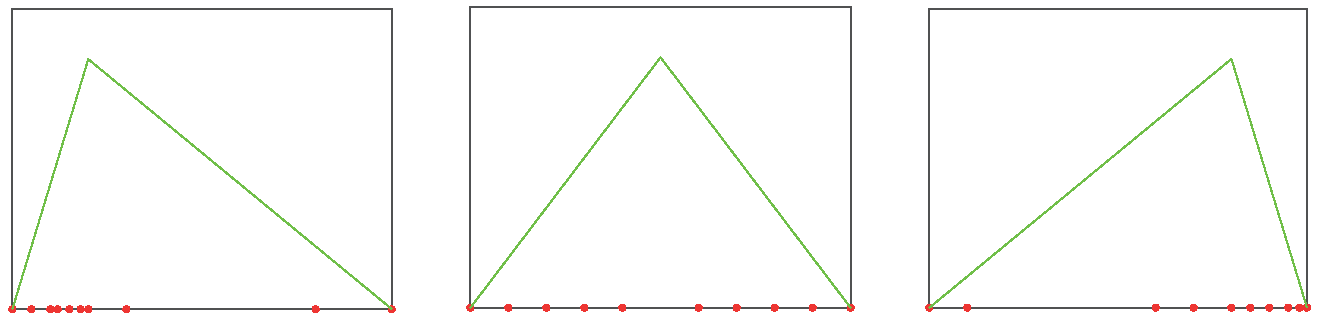
\includegraphics[width=0.9\textwidth]{compare_distribution}
    \caption{区间值相同但分布不同的数据比较}
    \label{fig:compare_distribution}
\end{figure}

\section{三角形模糊集值建模与相似性度量}
\label{sec:chap03-2}
当前,面向对象分割方法中对影像单元多采取均值数据建模 \cite{yu2012method} 和区间值数据建模 \cite{he2016remote} 。然而,这两种信息表达模型无法区分具有相同均值和区间值但内部分布不一致的分割单元。如图 \ref{fig:compare_distribution} 所示,三组模拟数据内的点看作一个影像分割单元像素点集合,具有相同的均值和区间值的影像单元内像素点的分布差异明显。

模糊集(Fuzzy sets, FS) 是 Zadeh 教授 1965年提出的概念,通过建立适当的隶属度函数(Membership function, MF)来描述对象的不确定性 \cite{zadeh1965fuzzy}。 常见的隶属度函数有:三角形MF,梯形MF,截断高斯MF和钟形MF等。 FS 最常用和最基本的 MF 是三角形MF。 因此,文中利用三角形模糊集来定义三角形模糊集值数据模型。

\begin{definition}
    三角形模糊集值模型的定义
\end{definition}
三角形模糊集值数据由以下三个关键参数组成:$(a^-,0)$,$(a^m,1)$ 和 $(a^+,0)$。如图~\ref{fig:tfs} 所示,  几何上,$(a^-,0)$ 和 $(a^+,0)$ 组成三角形MF的下边缘;代数上,$(a^-,0)$ 和 $(a^+,0)$ 形成一个区间值,确保一定的变化范围。$(a^m,1)$是三角形模糊集值数据的顶点,表征 FS 的最高置信度。

\begin{figure}[!htb]
    \centering
    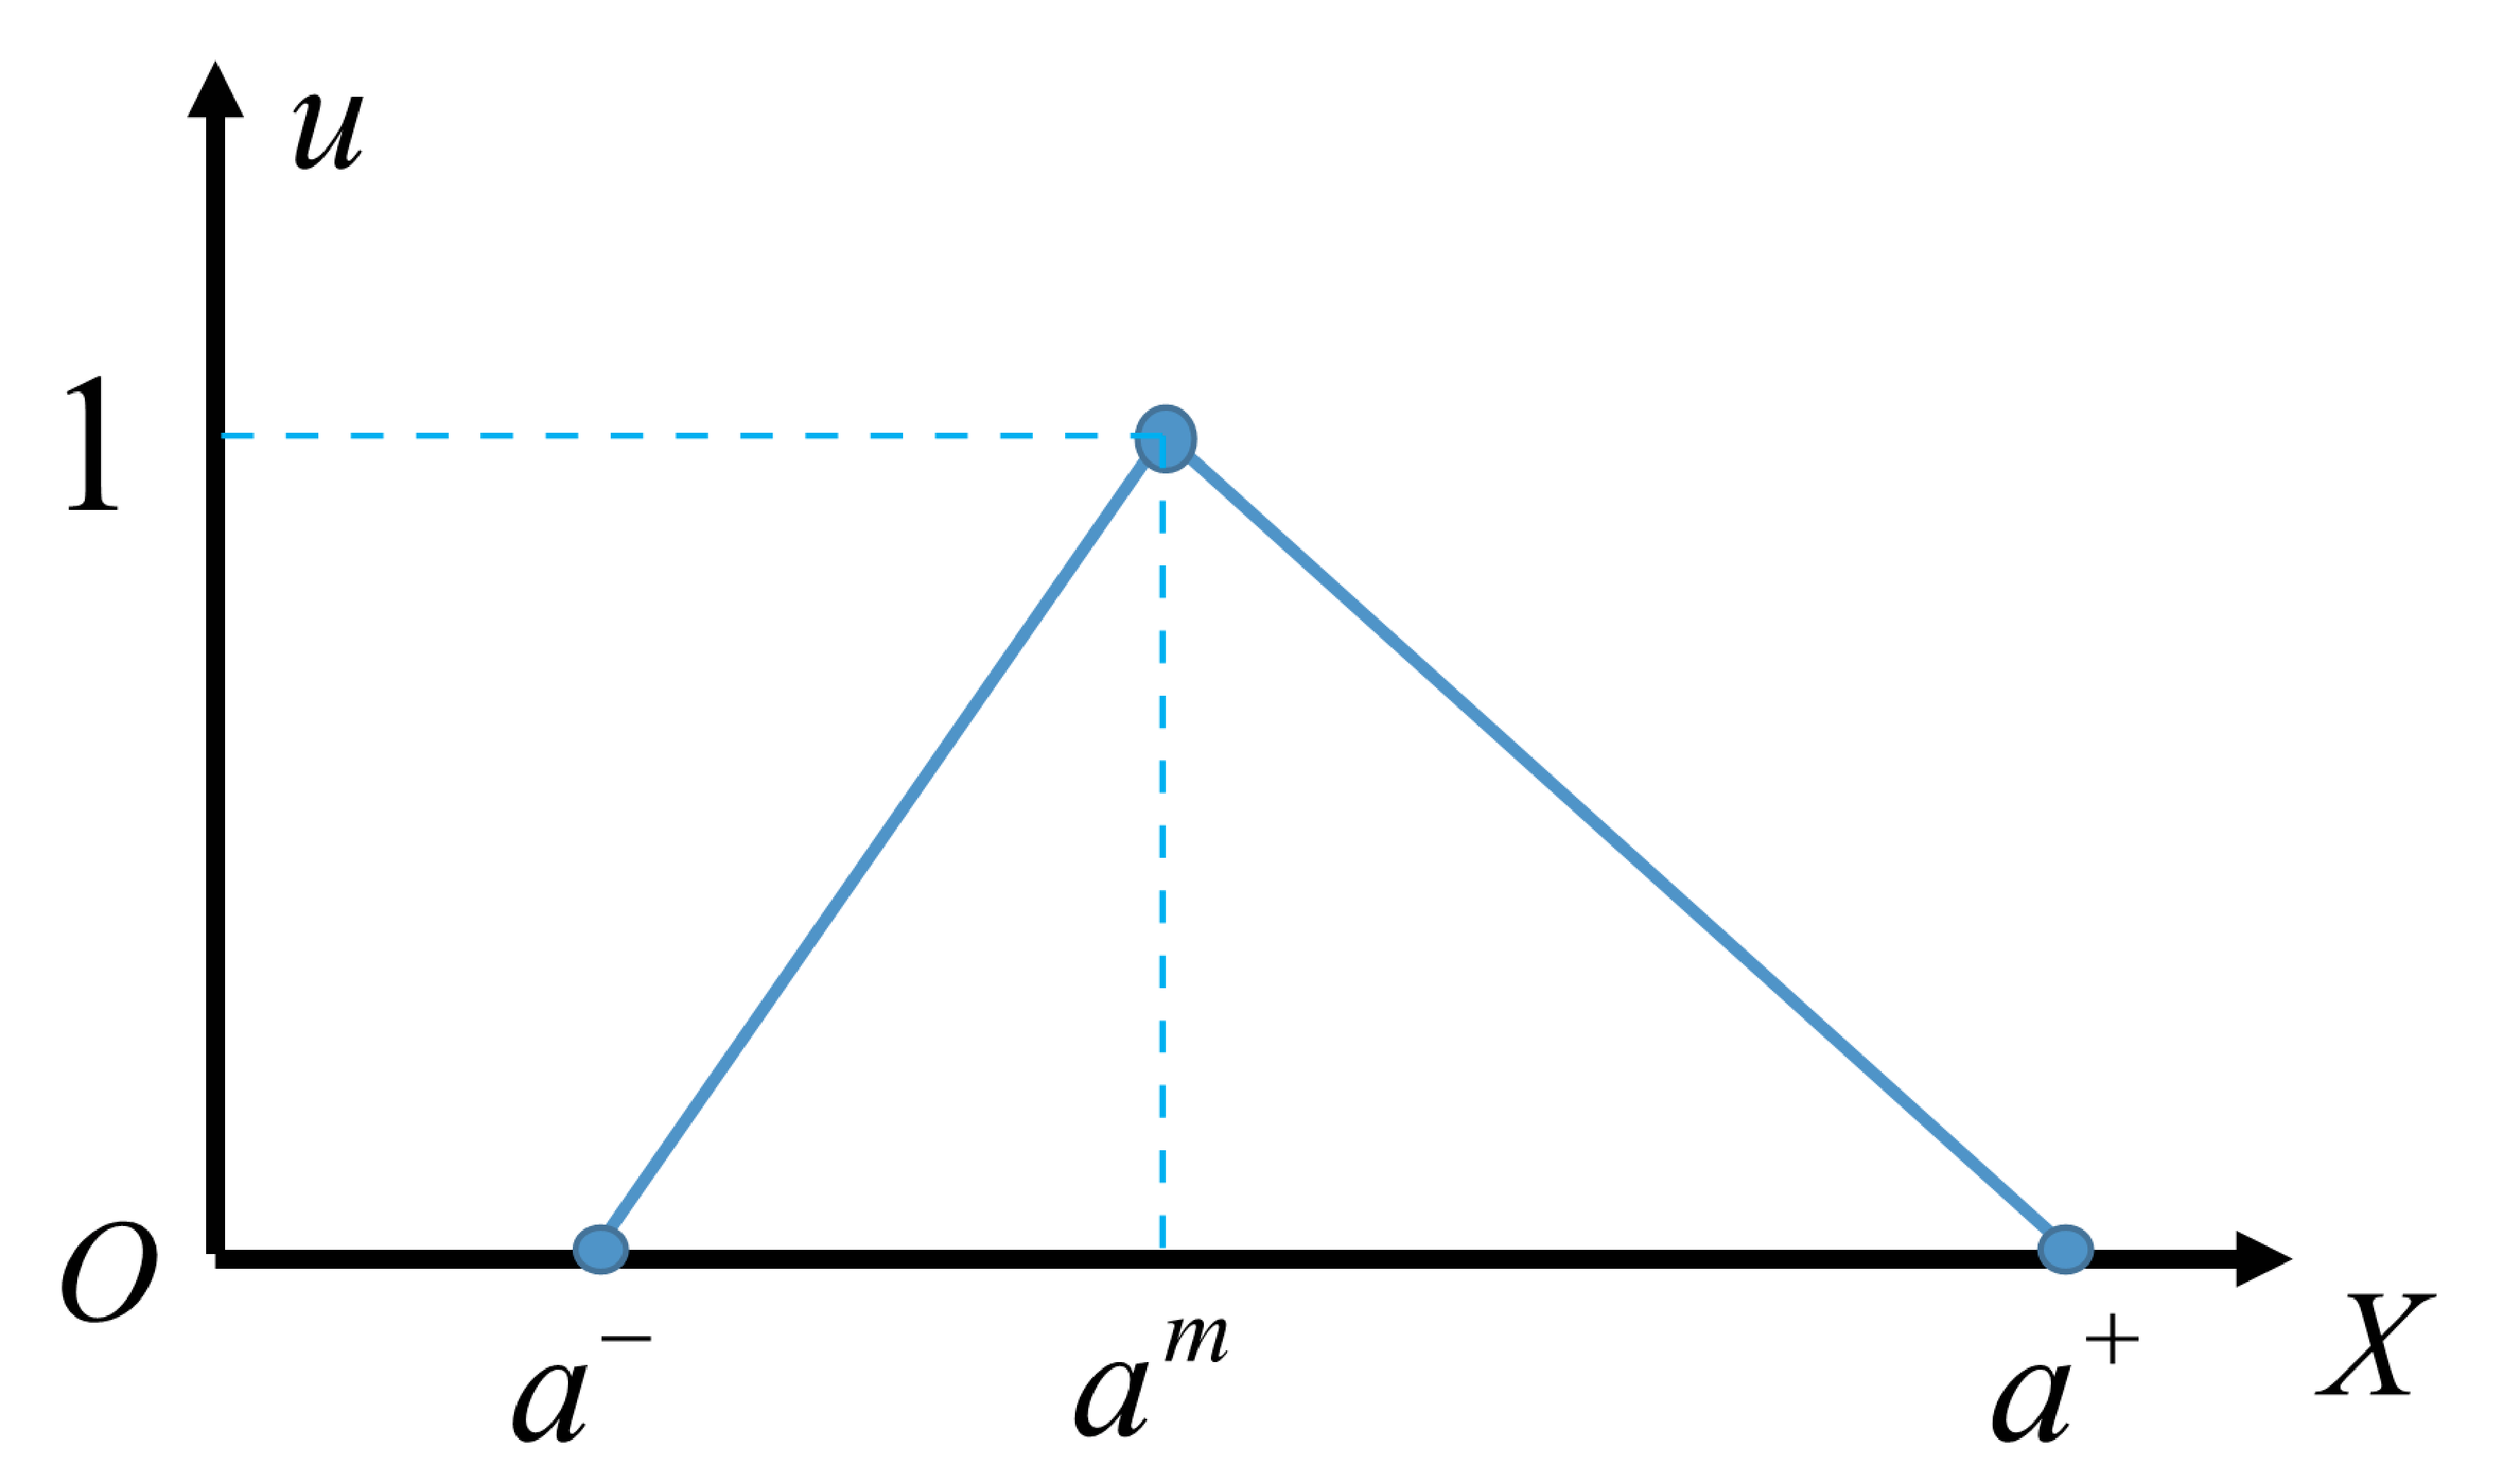
\includegraphics[width=0.5\textwidth]{tfs}
    \caption{三角形模糊集 $\tilde{A}$ 示意图}
    \label{fig:tfs}
\end{figure}

聚类是根据某种相似性或距离将相似的对象聚为一类的无监督学习方法,相似性度量是聚类的核心要素。对于两个三角形模糊集型数据$\tilde{A}$ 和 $\tilde{B}$,常见的相似性方法有以下几种:
\begin{enumerate}[(1)]
    \item 欧式距离(Euclidean distance)

          \begin{equation}
              \label{equ:eucliden}
              d_E(\tilde{A}, \tilde{B}) = \sqrt{\int_X |\tilde{A}(x)-\tilde{B}(x)|^2dx }, x \in X
          \end{equation}
          $\tilde{A}$ 和 $\tilde{B}$ 的欧式距离 $d_E(\tilde{A}, \tilde{B})$ 被看作是集合对应元素差值平方的积分的平方根。
    \item 城市距离(City-block distance)

          \begin{equation}
              \label{equ:cityblock}
              d_C(\tilde{A}, \tilde{B}) = \int_X |\tilde{A}(x)-\tilde{B}(x)|dx , x \in X
          \end{equation}
          $\tilde{A}$ 和 $\tilde{B}$ 的欧式距离 $d_E(\tilde{A}, \tilde{B})$ 被看作是集合对应元素差值绝对值的积分。
    \item 切比雪夫距离(Tchebyshev distance)

          \begin{equation}
              \label{equ:tchebyshev}
              d_T(\tilde{A}, \tilde{B}) = \sqrt[\infty]{\int_X |\tilde{A}(x)-\tilde{B}(x)|^\infty dx }, x \in X
          \end{equation}
          $\tilde{A}$ 和 $\tilde{B}$ 的欧式距离 $d_E(\tilde{A}, \tilde{B})$ 被看作是集合对应元素差值积分的一个极限值。
    \item 豪斯多夫距离(Hausdorff distance)

          豪斯多夫距离最开始为区间或普通集合设计,两个普通集合 $A$ 与 $B$ 的豪斯多夫距离为:
          \begin{equation} \label{eq:haus1}
              d_H(A, B) = \max \Big  \lbrace \sup_{a \in A} \inf_{b \in B} \abs{a-b}, \sup_{b \in B} \inf_{a \in A} \abs{a-b} \Big  \rbrace
          \end{equation}
          将其推广到模糊集,可以考虑模糊集 $\tilde{A}$ 和 $\tilde{B}$的一个 $\alpha-cut$ 截集 $d_H^{\alpha} (\tilde{A}, \tilde{B})$,则有:
          \begin{equation}\label{eq:haus_alpha}
              \begin{split}
                  d_H^{\alpha} (\tilde{A}, \tilde{B}) = \max \Big \lbrace \sup_{a \in \tilde{A_{\alpha}}} \inf_{b \in \tilde{B_{\alpha}}} \abs{a-b}, \sup_{b \in \tilde{B_{\alpha}}} \inf_{a \in \tilde{A_{\alpha}}}
                  \abs{a-b} \Big \rbrace
              \end{split}
          \end{equation}
          又模糊集中,
          \begin{equation}\label{eq:haus_alpha2}
              \begin{split}
                  d_H^{\alpha} (\tilde{A}, \tilde{B}) = \max \Big \lbrace \max_{a \in \tilde{A_{\alpha}}} \min_{b \in \tilde{B_{\alpha}}} \abs{a-b}, \max_{b \in \tilde{B_{\alpha}}} \min_{a \in \tilde{A_{\alpha}}} \abs{a-b} \Big \rbrace
              \end{split}
          \end{equation}
          然后对所有可能的$\alpha-cut$ 截集积分,就可得到模糊集 $\tilde{A}$ 和 $\tilde{B}$的豪斯多夫距离:
          \begin{equation}\label{eq:haus2}
              \begin{split}
                  d_H(\tilde{A}, \tilde{B}) = \int_0 ^1 d_H^{\alpha} (\tilde{A}, \tilde{B}) d \alpha = \int_0 ^1 \max \Big \lbrace \max_{a \in \tilde{A_{\alpha}}} \min_{b \in \tilde{B_{\alpha}}} \abs{a-b}, \max_{b \in \tilde{B_{\alpha}}} \min_{a \in \tilde{A_{\alpha}}} \abs{a-b} \Big \rbrace  d \alpha
              \end{split}
          \end{equation}
\end{enumerate}










\section{字体命令}
\label{sec:first}

苏轼(1037-1101),北宋文学家、书画家。字子瞻,号东坡居士,眉州眉山(今属四川)人
